% =========================================================
%  REPORT TEMPLATE — Theme 3B, Mathematical Formalisation with Lean
%
%  Compile with xelatex, not pdflatex. The Lean symbols (ℕ, ∑, ∈)
%  need it.
%
%  This is here to save you the setup time, nothing else. Only the
%  introduction is named. The rest is up to you, and how you organise
%  the report is part of what I mark. Add and remove sections as you
%  need.
%
%  Three things have to be in: individual reflections, a contribution
%  statement, and an AI-use statement from each of you.
%
%  The last section shows what you can use — Lean code, theorems,
%  boxes, a table. Take what you want, then delete it.
%
%  Change anything you like: colours, margins, fonts, the boxes. Or
%  start from your own preamble if you prefer.
% =========================================================
\documentclass[11pt,a4paper]{article}

\usepackage[margin=2.4cm]{geometry}
\usepackage{fontspec}
\setmonofont{DejaVu Sans Mono}[Scale=0.85]
\usepackage{amsmath,amssymb,amsthm}
\usepackage{booktabs}
\usepackage{enumitem}
\usepackage{xcolor}
\usepackage{graphicx}
\usepackage{tikz}
\usepackage{listings}
\usepackage[most]{tcolorbox}
\usepackage[hidelinks]{hyperref}
\urlstyle{tt}

% ---- Lean code ----
\definecolor{keywordcolor}{rgb}{0.4,0.1,0.5}
\definecolor{commentcolor}{rgb}{0.3,0.5,0.3}
\lstdefinelanguage{lean}{
  keywords={theorem,lemma,example,def,by,intro,exact,apply,rw,rfl,induction,
    cases,rcases,rintro,constructor,use,have,show,calc,ring,ring_nf,linarith,
    norm_num,simp,omega,sorry,fun,obtain,rwa,import,namespace,end,open,variable},
  sensitive=true, comment=[l]{--}, morecomment=[s]{/-}{-/},
  keywordstyle=\color{keywordcolor}\bfseries,
  commentstyle=\color{commentcolor}\itshape,
}
\lstset{language=lean, basicstyle=\ttfamily\small, columns=fullflexible,
  keepspaces=true, breaklines=true, frame=single, framerule=0.3pt,
  rulecolor=\color{black!30}, xleftmargin=1em, aboveskip=0.8em, belowskip=0.8em}

% \lean{...} for a Lean name inside a sentence: \lean{Finset.sum\_range\_succ}
\newcommand{\lean}[1]{\texttt{#1}}

\newtheorem{theorem}{Theorem}
\newtheorem{lemma}[theorem]{Lemma}
\newtheorem{definition}[theorem]{Definition}

% ---- Two boxes, shown in the last section ----
% These two hex codes set the box colours. Change them. Bristol red is
% {HTML}{B01B2E}.
\definecolor{boxmain}{HTML}{2F6FB3}
\definecolor{boxaccent}{HTML}{F2A900}
% \begin{keybox}{Title} ... \end{keybox}   — something to single out
\newtcolorbox{keybox}[1]{enhanced, colback=boxmain!6, colframe=boxmain,
  boxrule=0.7pt, arc=1mm, left=2mm, right=2mm, top=1.2mm, bottom=1.2mm,
  title={#1}, coltitle=white, colbacktitle=boxmain, fonttitle=\bfseries}
% \begin{notebox} ... \end{notebox}        — an aside, no title
\newtcolorbox{notebox}{enhanced, colback=boxaccent!12,
  colframe=boxaccent!70!black, boxrule=0.6pt, arc=1mm,
  left=2mm, right=2mm, top=1.2mm, bottom=1.2mm}

\title{\textbf{<Title of your result>}\\[0.3em]
  \normalsize Theme 3B --- Mathematical Formalisation with Lean}
\author{<Name> \and <Name> \and <Name>}
\date{}

\begin{document}
\maketitle

% ---------------------------------------------------------
%  Your report. Name the sections yourself.
% ---------------------------------------------------------

\section{Introduction}

\section{<Title>}

\section{<Title>}

\section{<Title>}

\begin{thebibliography}{9}
% One entry per source you actually read. Mathlib pages and search
% tools count. Cite the page, not the whole library.
\bibitem{ref1} <Author>, \emph{<Title>}, <year>.
\end{thebibliography}

% ---------------------------------------------------------
%  These three are required. Write your reflection yourself and
%  sign it.
% ---------------------------------------------------------

\section{Individual reflections}

\paragraph{<Name>.} % \hfill \emph{signed: <initials>}

\appendix

\section{Contribution statement}

% Who did what, agreed by all of you. One line each is enough.
\begin{center}
\begin{tabular}{@{}lp{11.5cm}@{}}
\toprule
\textbf{Member} & \textbf{Main contribution} \\
\midrule
<Name> &  \\
<Name> &  \\
<Name> &  \\
<Name> &  \\
<Name> &  \\
\bottomrule
\end{tabular}
\end{center}

\noindent % Say here that you all agree the statement, and sign it.

\section{AI-use statements (per member)}

% =========================================================
%  Below is just a show of what you can use. None of it is a model
%  answer. Take what is useful and DELETE THIS WHOLE SECTION.
% =========================================================
\section{What you can use (delete this section)}

Theorem, lemma and definition environments are defined. Label them and refer
back with \lean{\textbackslash ref}, as in Theorem~\ref{thm:example}.

\begin{theorem}\label{thm:example}
For every $n \in \mathbb{N}$, \quad
$\displaystyle\sum_{k=0}^{n-1}(2k+1) = n^2$.
\end{theorem}

\begin{proof}[Proof of Theorem~\ref{thm:example}, by induction on $n$]
The base case is the empty sum. For the step, $d^2 + (2d+1) = (d+1)^2$.
\end{proof}

Lean code goes in \lean{lstlisting}, which keeps the symbols intact:

\begin{lstlisting}
theorem my_result (n : ℕ) : ∑ k ∈ range n, (2 * k + 1) = n ^ 2 := by
  induction n with
  | zero => simp
  | succ d hd => sorry
\end{lstlisting}

For a Lean name inside a sentence use \lean{\textbackslash lean\{...\}},
giving \lean{Finset.sum\_range\_succ} --- note the backslash before the
underscore.

Two boxes; the colours are only a suggestion:

\begin{keybox}{The remaining obstacle}
Every odd $m < 2n$ must be shown to equal $2k+1$ for some $k < n$.
\end{keybox}

\begin{notebox}
In $\mathbb{N}$, subtraction truncates: $2 \cdot 0 - 1 = 0$, not $-1$.
\end{notebox}

A table, here recording who led on what and what was reused:

\begin{center}
\small
\begin{tabular}{@{}llll@{}}
\toprule
\textbf{Declaration} & \textbf{Lead} & \textbf{Status} & \textbf{Built or reused?} \\
\midrule
\lean{step}      & <name> & proved & built (\lean{ring}) \\
\lean{main\_thm} & <name> & proved & built on \lean{sum\_range\_succ} \\
\bottomrule
\end{tabular}
\end{center}

And a figure, from an image file or drawn with \lean{tikz}:

\begin{figure}[ht]
  \centering
  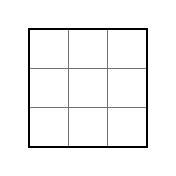
\begin{tikzpicture}[x=0.5cm,y=0.5cm]
    \draw[step=1,black!55,thin] (0,0) grid (3,3);
    \draw[black,thick] (0,0) rectangle (3,3);
  \end{tikzpicture}
  \caption{A caption.}\label{fig:example}
\end{figure}

\end{document}

